\chapter{Les relations entre chrétiens et musulmans
entre XIe et XVe siècles}

\mn{Marie Carmen Seance 6 28/02}


Une seance sera dédiée à l'empire Ottoman.

\section{La fragilisation du monde musulman oriental}


 Il ne faut pas parler de déclin car une période très prospère, avec des grands savants (Averroes, Al-Ghazali\sn{\textit{Statut de dimmi dans l'oeuvre d'Al Ghazali }par Emmanuel Pisani}, .

 \paragraph{La vision du monde occidentale} Le géographe
Al Masu’di (Xe siècle
L’humeur
\begin{quote}
    L’humeur chaude
manque chez eux [les peuples du Nord] ; leurs
corps sont épais, leurs natures grossières, leurs manières rudes,
leurs intelligences affaiblies et leurs langues lourdes.[… ] Leurs
croyances religieuses manquent de solidité. […] Ceux qui sont le
plus au nord sont les plus sujets à la stupidité, à la grossièreté et
à l’abrutissement.\sn{Cité par Bernard Lewis,
Les Arabes dans l’histoire , Paris, Flammarion, « Champs », 1993, p. 202.}
\end{quote}

\paragraph{perte d'autorité centrale}

\paragraph{Perte de pouvoirs des califats}

\paragraph{Moindre prospérité économique} du fait de la réduction des échanges

\paragraph{des dépenses dispendieuses de la cour}

paragraph{Repères chronologiques}

\begin{itemize}
    \item 
Apogée
de l’Empire abbasside sous le règne d’ Harun al Rachid (786 809)
    \item 
Apogée de la puissance des Omeyyades en Espagne sous le règne du calife
Abd al Rahman III (912 961) => califat omeyyade en Espagne à partir du
Xe siècle
    \item 
Création de la dynastie fatimide en Tunisie à partir de 910 puis occupation
de l’Egypte en 956 => califat fatimide. Il disparaît en 1171.
    \item 
Sultanat
mamelouk en Egypte : 1260 1517
\end{itemize}



\subsection{L’Empire seldjoukide}

\paragraph{Mamelouk} les arabes connaissaient les turcs en ayant des troupes turcs, les \textit{mamelouks}. 

\paragraph{A la même époque, la tribu seljoukide} Ils se convertissent à l'islam. 
 \begin{figure}[h!]
\centering
\sidecaption{Florian Louis,
Atlas
historique du
Moyen Orient , Paris,
Autrement, 2020, p.
42.}
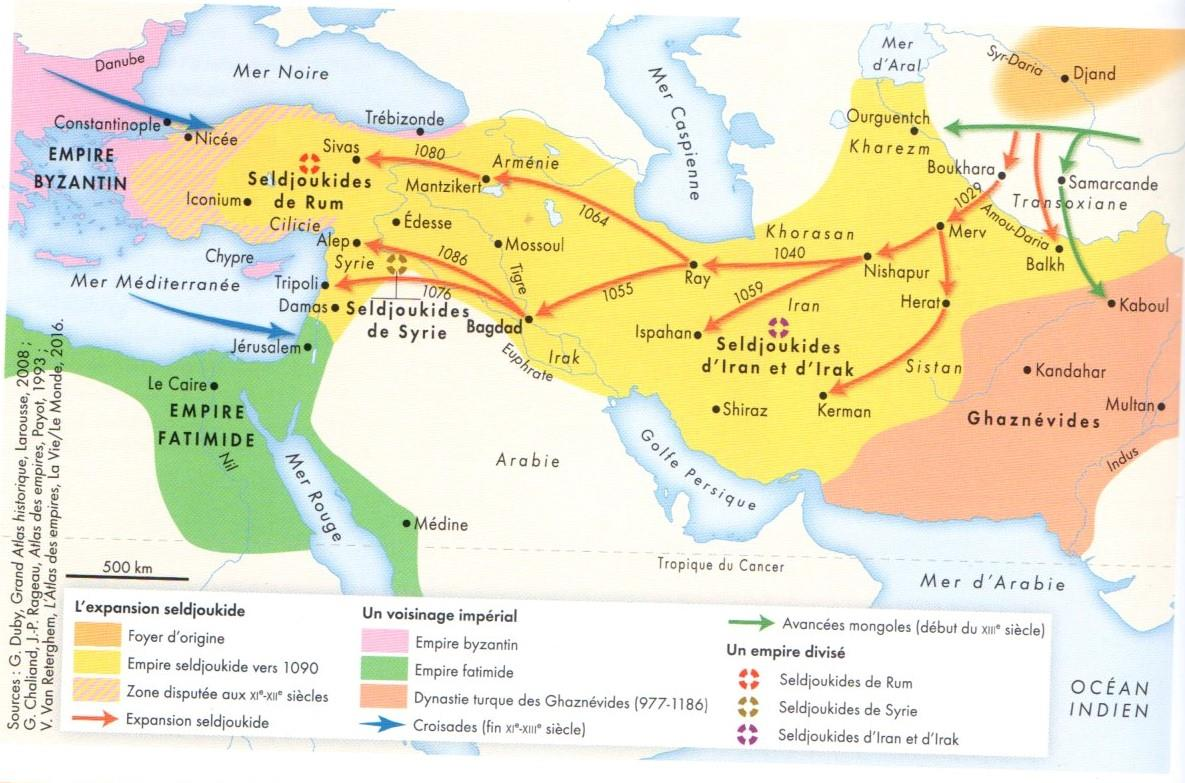
\includegraphics[width=\textwidth]{HistoireIslamMediterranee/Images/EmpireSeldjoukide.jpg}
     
     \label{fig:EmpireSldjoukide}
 \end{figure}

\paragraph{les principales batailles}

\begin{itemize}
    \item 1055
: Entrée de Tughrul bey dans
Badgad => titre de sultan seldjoukide
reçu de la main du calife.
    \item 1070
prise d’Alep
    \item 1071
: bataille de Manzikert; \textit{date importante} car une bataille contre les byzantins dans des terres traditionnellement byzantines. 
    \item 1074
: prise de Jérusalem
    \item 1078
: prise de Damas

\end{itemize}


 \paragraph{ Les règnes des 3 plus importants
sultans seldjoukides}
\begin{itemize}
    \item Tughrul
bey : 1055 1063
    \item Alp Arslan : 1063
1072
    \item Malik Shah : 1072
1092
\end{itemize}


\paragraph{Ils se convertissent par l'islam} soucis d'unification. 

\paragraph{Fragilisation de l'empire byzantins} les seljoukides ne pensaient pas les byzantins faibles. Or, en fait, l'empire byzantin est faible et les populations chrétiennes en Cappadoce et en Arménie ouvrent leurs villes aux Seljoukides.


\paragraph{Nizam al Mulk} Vizir iranien.
Dans le livre de Claude Cahen, il insiste sur l'originalité de l'empire seljoukide : bonnes conditions pour les chrétiens, mix iranien, Byzantin,... 
Beaucoup de constructions, caravanserails, les \textit{khans}. 

\paragraph{Developpement des madrasa} 

\paragraph{Bonnes relations chrétiennes} Plutot apaisées.
\paragraph{Ismaeliens}
on confond avec les fatimides.  En revanche, les ismaeliens vont être très intolérants vis à vis des seljoukides (en Syrie et Egypte). Ils sont connus sous le noms des \textit{Assassins}. Pas tellement contre les royaumes latins et les chrétiens (mais ils le seront aussi) mais surtout contre le pouvoir seljoukide. Or, on connaitra les assassins au XIII alors que les ismaeliens ne sont plus rien. \textit{Importance de la chronologie}

\paragraph{dislocation assez rapide à la fin du XI}

\subsection{Le lent déclin des Fatimides}

 \paragraph{Un descendant d'Ali et de Fatima} en Tunisie et en 969, vient au Caire. Va affronter l'empire Seljoukide. Ils prennent le terme d'Imam puis Calife.

 \paragraph{Califat sur le format de Bagdad} très efficace. Ils sont Ismaeliens chiites mais n'imposent pas leur religion.  

\paragraph{Economie florissante en s'appuyant sur les italiens} L'idée est de faire une deuxième route de la soie.

\paragraph{Al Häkim, une parenthèse très dure contre les chrétiens} Cloche autour du cou pour les chrétiens; pas de vins ni cochon, détruit les églises, dont le Saint Sépulcre et les synagogues.
A un moment, il arrête (fou ?). Il s'en va et ne revient pas. 

\paragraph{Empire disparaît sous les coups de Saladin en 1171} Saladin devient d'abord vizir des Fatimides. 

\subsection{Les Croisades}


Pise et Gênes commencent des pillages de terres musulmanes.
Reconquête de la Sicile par les Normands et début de la reconquête de l'Espagne.
\paragraph{Pourquoi les croisades ?}
Volonté certes de récupérer les lieux saints mais aussi de résister contre la pression seldjoukides. 
Mais il y a aussi d'autres causes : pacifier les querelles de chevaliers, comptoirs commerciaux italiens. 

 \begin{figure}[h!]
\centering
\sidecaption{Florian Louis,
Atlas historique du
Moyen Orient , Paris, Autrement,
2020, p. 40.}
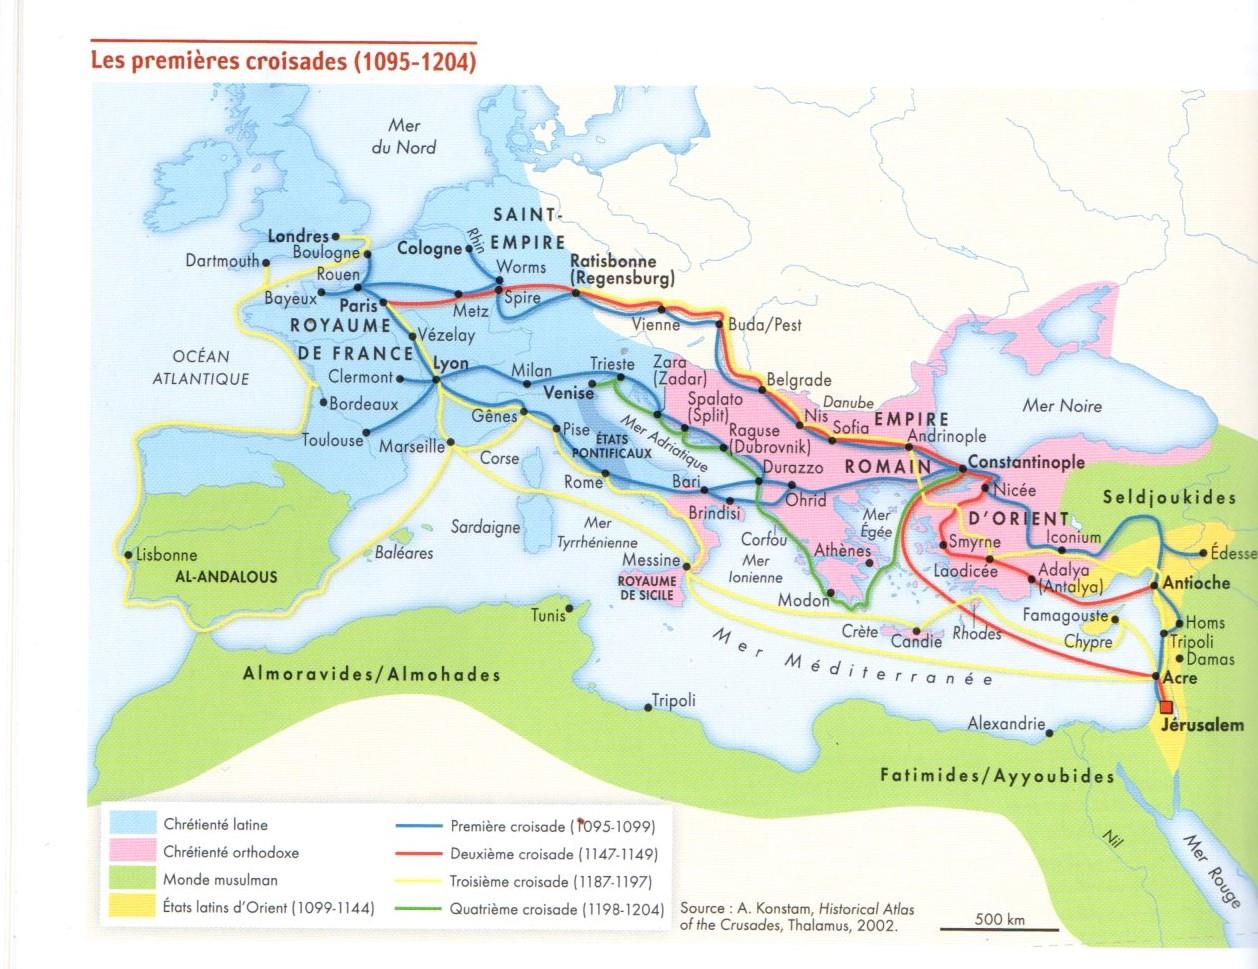
\includegraphics[width=\textwidth]{HistoireIslamMediterranee/Images/Croisade.jpg}
     
     \label{fig:Croisade}
 \end{figure}


\paragraph{Pour les musulmans, pas une compréhension rapide de la nouveauté des croisades} Une vision plutôt des mercenaires des byzantins.

\paragraph{statut des chrétiens remis en cause} Exécution préventive des chrétiens à Alep. Destruction des églises à Alep.


  \begin{figure}[h!]
\centering
\sidecaption{Florian Louis,
Atlas historique du Moyen Orient , Paris,
Autrement, 2020, p. 41.}
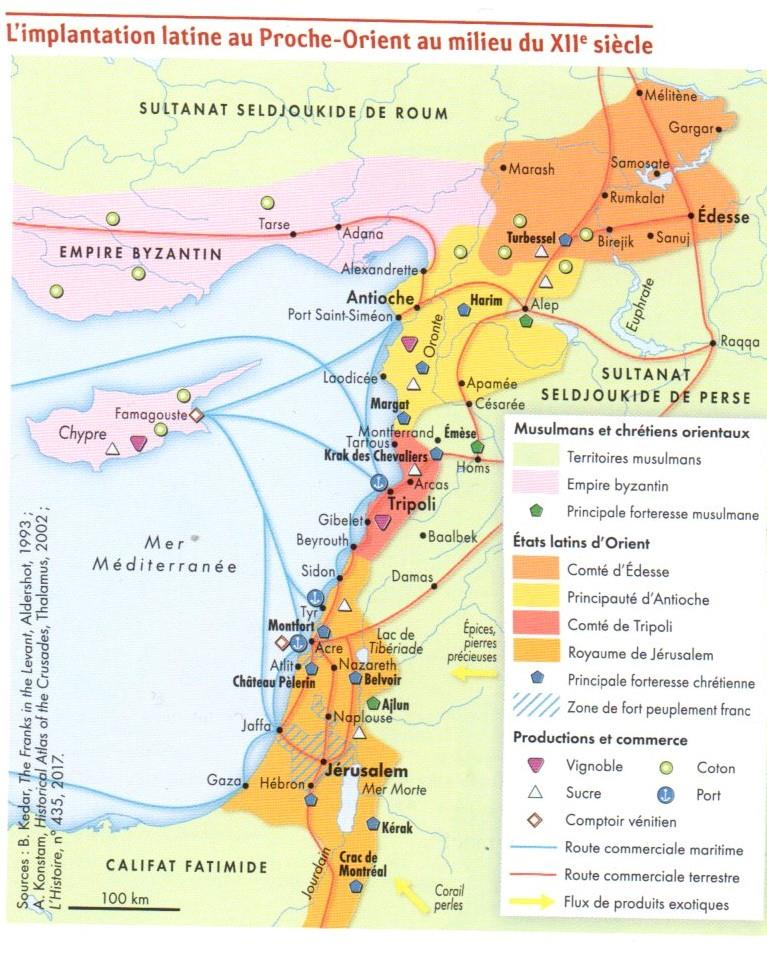
\includegraphics[width=0.8\textwidth]{HistoireIslamMediterranee/Images/Latin.jpg}
     
     \label{fig:Latin}
 \end{figure}


\paragraph{Tampon} entre Empire Seljoukide et Fatimide (au grand soulagement des Fatimides). 

\paragraph{Croisade, terme du XIII} Avant c'est une guerre

\paragraph{Repères chronologiques}
\begin{itemize}

    \item   1095
1099 : 1ere Croisade
    \item   1097
prise de Nicée et Edesse aux Seldjoukides
    \item   1099
prise de Jérusalem aux Fatimides
Création
de 4 Etats latins :
Royaume de Chypre
Royaume de Jérusalem
Principauté d’Antioche
Comté de Tripoli
    \item   
1147
1149 : 2eme Croisade
    \item  1154 : prise de Damas par Nur
al Din
    \item  1187
1197 3e Croisade
    \item  1187
prise de Jérusalem par Saladin, dynastie des Ayyoubides
Dynastie
des Ayyoubides règne en Syrie et en Egypte
=>
reconstitution du royaume de Jérusalem à Acre
    \item  1202
1204 : 4e Croisade (décidée dès 1198)
   \item  1204 : Sac de Constantinople
\item 1217
1221 : 5e Croisade
    \item  1227
1229 : 6e Croisade
    \item  1248
1254 : 7e Croisade
1263
    \item  1270 : 8e Croisade
1291 : 9e Croisade pour certains historiens
Prise de
Saint Jean d’Acre par les Mamelouks
\end{itemize}


\paragraph{Après la première phase de violence, une période calme} Les Chrétiens épousent des musulmanes qui se convertissent.
 \paragraph{Foucher
de Chartres, chroniqueur de la
première Croisade} 
\begin{quote}
  
Aujourd’hui, nous qui étions occidentaux sommes devenus orientaux.
Tel qui était italien ou français est
devenu galiléen ou palestinien dans ce pays. […] Nous avons presque oublié nos lieux de naissance. La
plupart d’entre nous ne les connaissent pas ou n’en ont pas même entendu parler. Celui ci possède
maison et propriété comme si c’était son héritage paternel ; tel autre a pris pour femme non point une
compatriote mais une Syrienne ou une Arménienne, voire même une Sarrasine baptisée.


[…] L’étranger est devenu un indigène, l’immigrant est à présent un résident. Chaque jour, nos parents et
nos amis suivent notre exemple abandonnant volontairement tout ce qu’ils possèdent en Occident.
Ceux qui étaient pauvres là bas, Dieu les fait riches ici. Celui qui n’avait que quelques sous là bas
possède ici d’innombrables pièces d’or et d’argent ; tel qui n’avait pas même un village possède ici, avec
l’aide de Dieu, une ville entière. Pourquoi donc retourner en Occident alors que l’Orient nous convient si
bien ? \mn{Cité par Bernard Lewis,
Les Arabes dans l’histoire , Paris, Flammarion, « Champs », 1993, p. 18 5}

\end{quote}


\paragraph{Réaction musulmane et 2ème croisade} avec un officier seljoukide \textit{Zangi}. Il va conquérir Mossul et il s'empare d'Edesse. 
Cela entraîne la deuxième croisade : 
\begin{itemize}
    \item 1147
1149 : 2eme Croisade
    \item  1154 : prise de Damas par Nur
al Din, fils de Zangi
\end{itemize}

\paragraph{Nur al Din va profiter de la faiblesse du califat fatimide } pour conquérir l'Egypte

\paragraph{Après les fatimides, les Ayyoubides et 3ème croisade} Califat ayyoubide créées par Saladin qui prend la Syrie et Jérusalem. La capital du Royaume Latin à Acre. 
3ème croisade, avec Richard Coeur de Lion et Philippe 
Auguste.

\paragraph{A la mort de Saladin} fragmentation de la syrie en principautés musulmanes mais Egypte reste solide. 

\paragraph{4ème croisade} Celle dont on se souvient le plus, sac de Constantinople; Partage des comptoirs byzantins entre vénitiens et génois. fracture des chrétiens. 

\subsection{Les Mongols}

\paragraph{Gengis Khan et l’invasion mongole}
\begin{itemize}
    \item 1166
: Naissance de Gengis Khan
    \item 1206
Gengis Khan reconnu Empereur par l’assemblée des Mongols
    \item 1221
: Conquête de l’Iran
    \item 1227
: Mort de Gengis Khan
    \item 1258
: prise de Bagdad et mort du Calife => abolition du califat abbasside de Bagdad
\end{itemize}

  \begin{figure}[h!]
\centering
\sidecaption{Florian Louis,
Atlas
historique du Moyen
Orient , Paris,
Autrement, 2020, p.
43.}
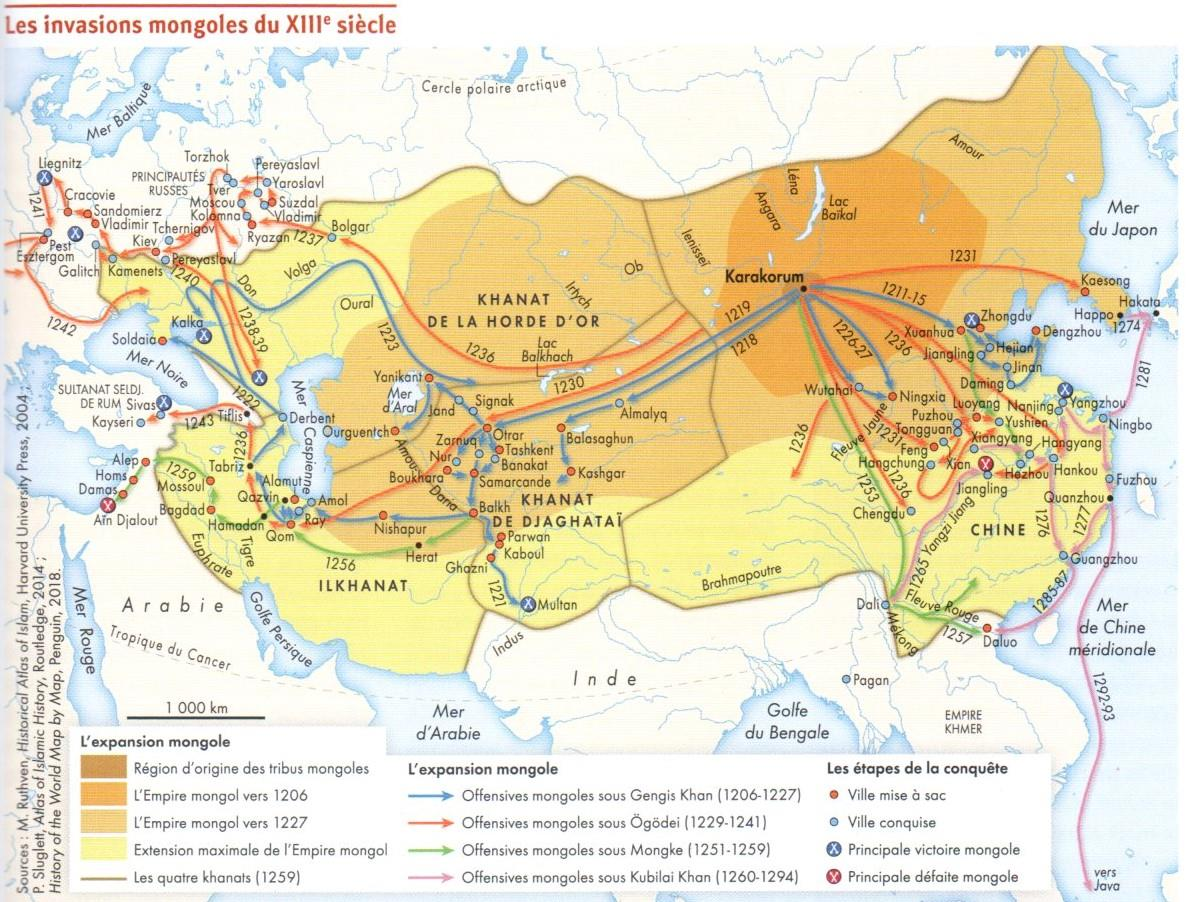
\includegraphics[width=\textwidth]{HistoireIslamMediterranee/Images/Mongol.jpg}
     
     \label{fig:Mongols}
 \end{figure}

 \paragraph{le centre de gravité de l'Empire Mongol sera l'Iran} S'ouvre au commerce. Conquiert la Syrie. Chrétiens et juifs au début plutôt accueillants.

 
\subsection{Le sultanat mamelouk}


\paragraph{le sultanat Ayyoubide disparait}

\paragraph{Importance des italiens} Période très intense culturelle : mosquée, madrasa,..

\paragraph{1275 : conquête des états latins} fin en 1291


\paragraph{Tamerlan, 13xx} depuis la capitale, Samarcande.
  \begin{figure}[h!]
\centering
\sidecaption{Florian Louis,
Atlas
historique du Moyen
Orient , Paris,
Autrement, 2020, p.
43.}
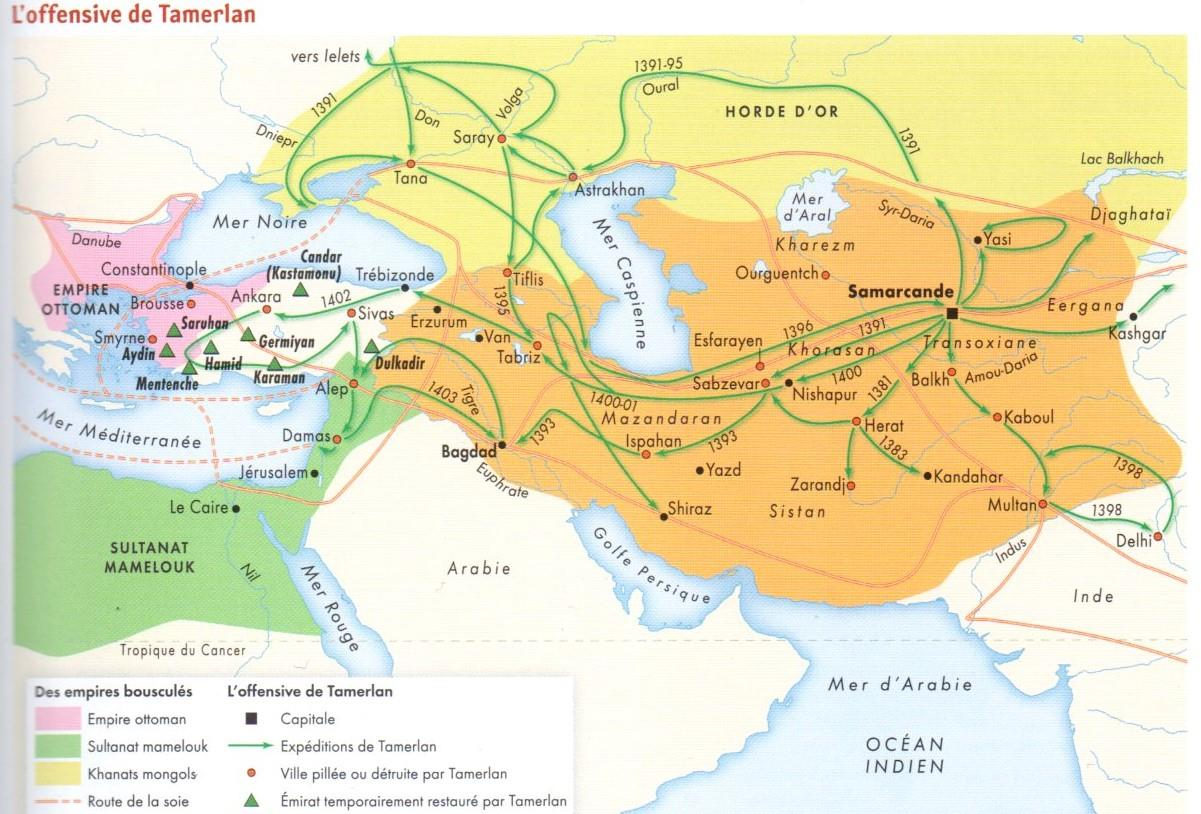
\includegraphics[width=\textwidth]{HistoireIslamMediterranee/Images/Tamerlan.jpg}
     
     \label{fig:Mongols}
 \end{figure}

\paragraph{des massacres chrétiens horribles} au nom de l'Islam, des chrétiens enterrés vivants.

\section{Musulmans et chrétiens en Occident}


\subsection{Al-Andalous}
\paragraph{Au XIIIe les Chrétiens sont inexistants} alors qu'ils étaient majoritaires au X. 

\paragraph{les taifas} principauté autonome

\paragraph{Chronologie de la reconquista}

\begin{itemize}
 
    \item 1085 : Tolède perdue par les musulmans
    \item 1212
défaite musulmane à Las Navas de Tolosa
    \item 1236 : perte de Cordoue par les troupes musulmanes
    \item 1248 : perte de Séville par les troupes musulmanes
    \item 1492 : les troupes du roi espagnol Ferdinand d’Aragon entrent dans Grenade
\end{itemize}

\paragraph{Des exactions contre les mosquées} Les mosquées de la ville sont transformées en Eglise. 

\paragraph{Des berbères Almoravides contre les Taifas} pour sauver l'empire . Bcp plus dur sur les non-musulmans. \sn{Spécialité de John Tolan} Impossibilité pour un musulman de s'occuper des latrines,...

\paragraph{Les Almohades} sont encore plus intolérants au point que les chrétiens partent du Maroc. En parallèle, Séville, magnifique.

\paragraph{Tjs compliqué : \textit{en même temps}} Il faut nuancer car les Almohades / Amohavides sont capables d'avoir des mercenaires chrétiens. 

\paragraph{Grenade} à la chute des Almohades. Le statut des musulmans est proche des \textit{dhimmis}. 

\paragraph{1492} prise de Grenade. Violence contre juifs et musulmans (vont au Maghreb).

\paragraph{Reconquista de la Sicile} mais contexte différent car la Sicile avait plus de la moitié des habitants qui étaient restés Chrétiens. On impose la \textit{dhimmi}. A partir du XII - XIII, texte juridique pour imaginer le statut légal du musulman : minorité religieuse mais pas sociale. Il y a de la ségrégation mais on ne veut pas qu'ils se convertissent. 


\section{Conclusion}

\begin{Synthesis}
\begin{itemize}
    \item La langue arabe cantonnée à la théologie et aux sciences et aux terres arabes.
\item parler de déclin est trop fort
\end{itemize}

\end{Synthesis}